%--------------------
% Packages
% -------------------
\documentclass[11pt,a4paper]{article}
\usepackage[utf8x]{inputenc}
\usepackage[T1]{fontenc}
%\usepackage{gentium}
\usepackage{mathptmx} % Use Times Font
\usepackage{amsmath}

\usepackage[pdftex]{graphicx} % Required for including pictures
\graphicspath{ {images/} }
\usepackage[pdftex,linkcolor=black,pdfborder={0 0 0}]{hyperref} % Format links for pdf
\usepackage{calc} % To reset the counter in the document after title page
\usepackage{enumitem} % Includes lists
\usepackage{listings}
\usepackage{xcolor}
\usepackage{hyperref}

\definecolor{codegreen}{rgb}{0,0.6,0}
\definecolor{codegray}{rgb}{0.5,0.5,0.5}
\definecolor{codepurple}{rgb}{0.58,0,0.82}
\definecolor{backcolour}{rgb}{0.95,0.95,0.92}

\lstdefinestyle{mystyle}{
    backgroundcolor=\color{backcolour},   
    commentstyle=\color{codegreen},
    keywordstyle=\color{magenta},
    numberstyle=\tiny\color{codegray},
    stringstyle=\color{codepurple},
    basicstyle=\ttfamily\footnotesize,
    breakatwhitespace=false,         
    breaklines=true,                 
    captionpos=b,                    
    keepspaces=true,                 
    numbers=left,                    
    numbersep=5pt,                  
    showspaces=false,                
    showstringspaces=false,
    showtabs=false,                  
    tabsize=2
}
\lstset{style=mystyle}

\frenchspacing % No double spacing between sentences
\linespread{1.2} % Set linespace
\usepackage[a4paper, lmargin=0.1666\paperwidth, rmargin=0.1666\paperwidth, tmargin=0.1111\paperheight, bmargin=0.1111\paperheight]{geometry} %margins
%\usepackage{parskip}

\usepackage[all]{nowidow} % Tries to remove widows
\usepackage[protrusion=true,expansion=true]{microtype} % Improves typography, load after fontpackage is selected

\counterwithin*{subsection}{section}
\renewcommand{\thesubsection}{\thesection.\alph{subsection}}

%-----------------------
% Set pdf information and add title, fill in the fields
%-----------------------


\hypersetup{ 	
pdfsubject = {Machine Learning 2 - Final Assignment},
pdftitle = {Machine Learning 2 - Final Assignment},
pdfauthor = {Frans de Boer}
}

\title{Machine learning 2 - Final Assignment}

\author{
    Frans de Boer \\
    fransdeboer \\
    5661439 \\
}

%-----------------------
% Begin document
%-----------------------
\begin{document} %All text i dokumentet hamnar mellan dessa taggar, allt ovanför är formatering av dokumentet
\maketitle

The git repository for this assignment with the code and the report can be found at \url{https://github.com/Frans-db/ml2.final-assignment}. I will make this repository public after the Brightspace deadline has passed.

\section{PAC Learning}

\subsection{Extend the proof that was given in the slides for the PAC-learnability of hyper-rectangles:
show that axis-aligned hyper-rectangles in n-dimensional feature spaces (n > 2) are PAC
learnable.}
  
We can extend the proof by taking the number of sides/faces of the hyper-rectangle into account.
\begin{itemize}
    \item A hyper-rectangle in 2-dimensional space is simply a rectangle and has 4 sides.
    \item A hyper-rectangle in 3-dimensional space is a rectangular box and has 6 sides.
\end{itemize}
For now I will assume the number of sides on a n-dimensional hyper-rectangle to be $F(n)$, and I will get back later to the calculation of $F(n)$.

To start we can follow the steps from the lecture. We have the ground truth n-dimensional hyper-rectangle $R$, and the current tightest fit rectangle $R'$. The error ($R - R'$) can be split into $F(n)$ strips $T'$. On each of these strips we can now grow a new strip $T$ such that the probability mass of $T$ is $\frac{\epsilon}{F(n)}$.

If $T$ covers $T'$ for all strips then the probability of an error is
\begin{equation}
    \label{eq:total_error}
    P[error] \leq \sum_{i=0}^{F(n)-1}P[T_i] = F(n)\frac{\epsilon}{F(n)} = \epsilon
\end{equation}

We can now estimate the probability that $T$ does not cover $T'$

\begin{align*} 
    &P[\textit{random x hits T}] = \frac{\epsilon}{F(n)} \\
    &P[\textit{random x misses T}] = 1 - \frac{\epsilon}{F(n)} \\
    &P[\textit{m random x's misses T}] = (1 - \frac{\epsilon}{F(n)})^m \\
\end{align*}

Since we have $F(n)$ strips:
\begin{align*} 
    &P[\textit{m random x's miss any Ts}] \leq F(n) (1 - \frac{\epsilon}{F(n)})^m \\
    &P[\textit{R' has larger error than } \epsilon] \leq F(n) (1 - \frac{\epsilon}{F(n)})^m\ < \delta \\
\end{align*}

Bounding the chance that our R' has an error larger than $\epsilon$ by $\delta$:

\[F(n) (1 - \frac{\epsilon}{F(n)})^m\ < \delta\]
Using $e^{-x} \geq (1-x)$
\[F(n)e^{-m\epsilon / F(n)} \geq F(n)(1 - \frac{\epsilon}{F(n)})^m\]
So instead we can use:

\begin{align*} 
    &F(n)e^{-m\epsilon / F(n)} < \delta \\ 
    &-m\epsilon / F(n) < \log{(\delta / F(n))} \\
    &m\epsilon / F(n) > \log{(F(n) / \delta)} \\
    &m > (F(n) / \epsilon)\log{(F(n) / \delta)} \\
\end{align*}

So any n-dimensional hyper-rectangle is learnable.

\subsection{Assume we have a 2-dimensional feature space R2, and consider the set of concepts that are L1-balls: $c = \{(x, y) : |x| + |y| ≤ r\}$ (basically, all L1-balls centered around the origin). Use a learner that fits the tightest ball. Show that this class is PAC-learnable from training data of size m.}
\label{sec:2b}

Same thing? what. literally just question a but now rotated 45 degrees

\subsection{Now we extend the previous class by allowing the varying center: $c = \{(x, y) : |x − x0| + |y − y0| ≤ r\}$. Is this class PAC-learnable? Proof if it is, or otherwise disproof it.}
\label{sec:2c}

This is just a generalization of Section \ref{sec:2b}, but now with a varying center. Our hypothesis space is still a tightest fit ball around the sampled data, which will now also be shifted by $(x_0, y_0)$. Since we are still dealing with a consistent learner this class is also PAC-learnable.

The worked out proof for this is the same as for Section \ref{sec:2b}.

\subsection{Generate data according to, what you would argue is, the ‘best case’ scenario, i.e., for
which learning is easiest. Clearly specify how you generate this data and show the resulting
learning curve.}

First I'll discuss the setup I'm using to run these tests. I'm generting $L_1$ balls with $r=1$. I've set the size of the sample space to 2. This means that the sample space is a $2x2$ square with the center at $(0,0)$. The surface area of this square is $4$, and the surface area of the $L_1$ ball is $2$, exactly half of the sample space.

For each tests I'll be using a sample size of $m \in \{2, ... , 10000 \}$, and I'll be taking the average of 100 trials. From a set of samples $m$ the surface area of the  $L_1$ ball can be determined, and from here the error of the ground truth can be calculated. This error is 

\[(2 - \textit{estimated\_area}) / 2\]

$2$ is the surface area of the ground truth $L_1$ ball. This is divided by 2 because only positive samples that fall into this area will be misclassified (negative samples are never misclassified).

First I wanted to run a test using a basic uniform distribution to confirm the code is working properly. The results from this test can be seen in Figure \ref{fig:learningcurve_uniform}. The more samples get added, the lower the error will be.

\begin{figure}[h]
    \caption{Learning Curve for a points sampled from a uniform distribution}
    \centering
    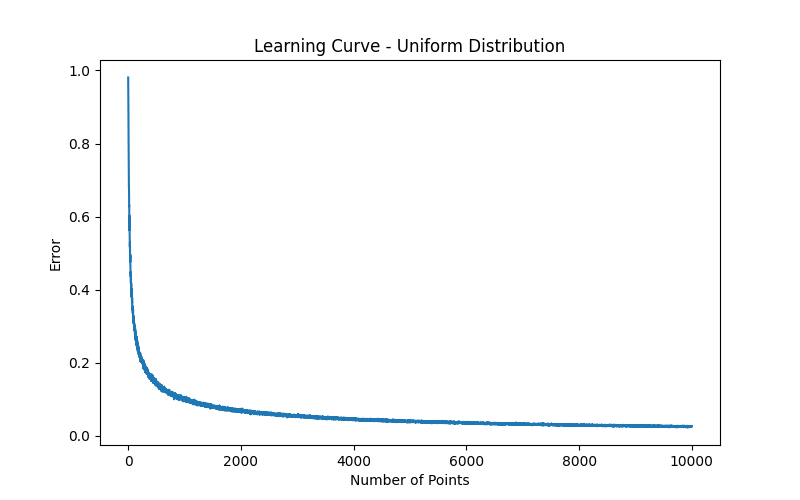
\includegraphics[width=\textwidth]{learningcurve_uniform.png}
    \label{fig:learningcurve_uniform}
\end{figure}

I personally think the best case scenario would be a method that generates samples close to the edge of the $L_1$ ball. To do this I generated values for polar coordinates and converted these to cartesian coordinates in the following way:

\begin{align*} 
    &r_i ~ N(1, 0.2) \\ 
    &d_i ~ U(0, 2\pi) \\
    &x_i = r_i \cos(d_i) \\
    &y_i = r_i \sin(d_i) \\
\end{align*}

This will generate samples following a donut like distribution (see Figure \ref{fig:donut} for an example of generated points). The learning curve can be seen in Figure 

\begin{figure}[h]
    \caption{Donut Distribution ($m=10000$)}
    \centering
    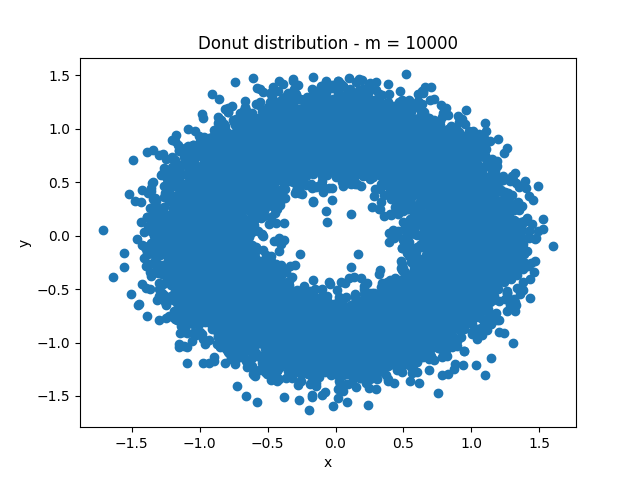
\includegraphics[width=\textwidth]{donut.png}
    \label{fig:donut}
\end{figure}

\subsection{Similarly, generate data according to, what you would argue is, the ‘worst case’ scenario.
Clearly specify how you generate this data and show the resulting learning curve. How
close is this curve to the theoretical PAC bound?}


\clearpage
\section{VC Dimension}
\label{sec:VC}
Let us assume we are dealing with a two-class classification problem in d-dimensions.
Let us start off with refreshing our memories. Consider the class of linear hypotheses (i.e.,
all possible linear classifiers) in d-dimensional space.

\subsection{Given N data points, how many possible labelings does this data set have?}
\label{sec:2a}
Each data point can have 2 labels, so $2^N$

\subsection{What is the dimensionality d we need, at the least, for our class of linear hypotheses to
be able to find perfect solutions to all possible labelings of a data set of size N? Stated
differently, what is the smallest d that allows us to shatter N points?}
\label{sec:2b}

From the \textit{Machine Learning 1} course (2021/22 edition, Week 4: Complexity and SVMs): A linear classifier with $d$ parameters (dimensions) can shatter $d+1$ points. In other words, the smallest $d$ that allows us to shatter $N$ points is $d = N - 1$. 

\subsection{Consider d = 1 and a data set of size N. At maximum, how many different labelings of
such a data set can decision stumps solve perfectly, i.e., with zero training error?}
\label{sec:2c}
This would be all cases where there is no overlap, i.e. all points with class 1 (or 2) are either all on the left or right side. See Figure \ref{fig:d1n3} for an example with N=3. Note that the first 3 and last 3 examples are the same, just with inverted labelings.

\begin{figure}[h]
    \caption{Example of perfectly solvable labels with $N=3$}
    \centering
    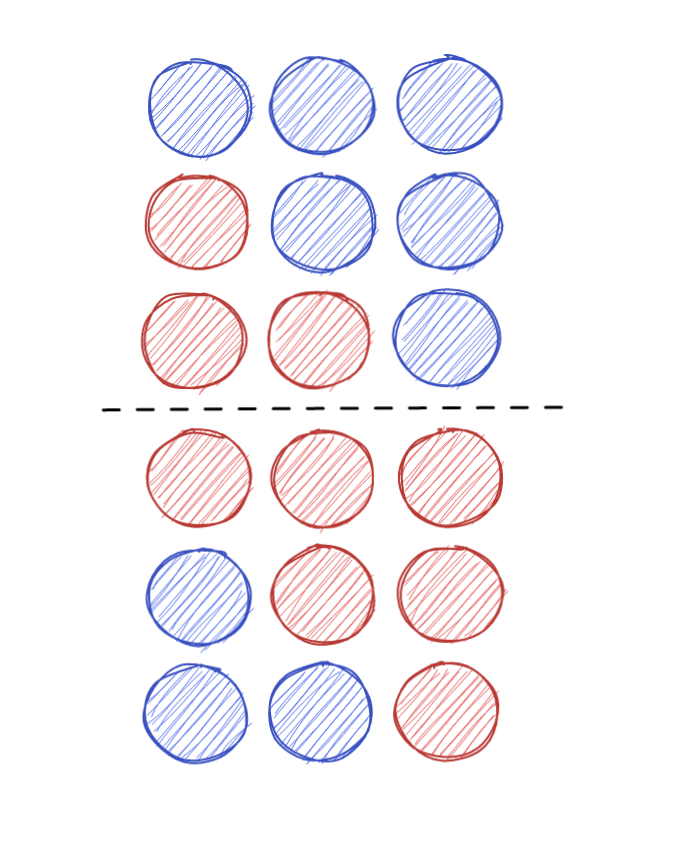
\includegraphics[width=0.5\textwidth]{d1n3_possibilities.png}
    \label{fig:d1n3}
\end{figure}

With a dataset of size N, there are N ways in which we can have class 1 be on the left side and have a decision stump be able to solve it perfectly. There can be $1, 2, ..., N$ points with class 1 in a row.
Because each of these possible label assignments has a compliment (just invert the classes), we end up with a total of $2N$ possible labelings that a decision stump can solve perfectly.


\subsection{With the answer from 3.c, give an upper-bound on the maximum number of different
labelings a data set of size N in d dimensions can get by means of decision stumps.}
\label{sec:2d}

We can once again look at Figure \ref{fig:d1n3}, but now instead of true labels we can view the labels (red and blue) as labels predicted by the decision stump. The decision stump either assigns all points to the left of it as class 1 or as class 2. So in $d=1$ we know the maximum number of different labelings a data set of size N can get is $2N$. 

This can be viewed in another way, for every dimension the decision stump can make $2N$ different labelings. For example in 2D (Figure \ref{fig:d2n3}) the decision stump for the x dimension can make $2N$ labelings, and the decision stump for the y dimension can make $2N$ labelings.

This continues for each dimension added, so we end up with a total of $2Nd$ maximum number of different labelings a data set of size N in d dimension can get by means of decision stumps.


\begin{figure}[h]
    \caption{Example with $d=2$ and $N=3$}
    \centering
    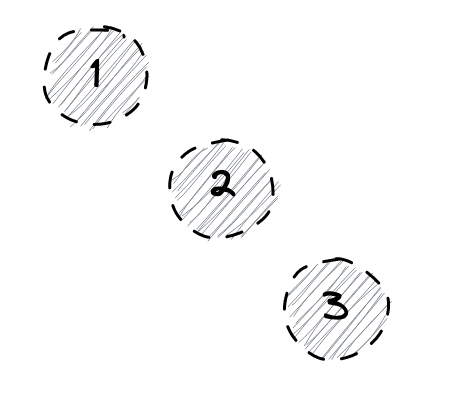
\includegraphics[width=0.5\textwidth]{d2n3_unlabeled.png}
    \label{fig:d2n3}
\end{figure}

I'd like to add some more notes to this solution. This is not neccesary to read, but it sheds some light on some of the mistakes I made. 

While trying to answer this question I pretty quickly came to the answer of $2Nd$, but then later thought it to be wrong because this formula does not take into account duplicate labelings. In Figure \ref{fig:d2n3} for example the x and y decision stumps can create many duplicate label assignments. 

I tried to find patterns in combinations of $N$ and $d$, for example I noticed that for $d=2$ only $N \leq 3$ was solvable (see Figure \ref{fig:d2n3_solvable}), and for $d=3$ at least $N \leq 4$ was solvable (see Figure \ref{fig:d3n4_solvable}, here smaller circles can be seen as being further away in the z dimension). 

From here it seemed like there was a pattern where for any $N \leq (d+1)$ the problem was fully solvable, so the number of possible labelings the decision stump could make was $2^N$. I could however not find a pattern in the number of labelings a decision stump could make for problems with $N > (d+1)$.

\begin{figure}[h]
    \caption{Solvable example with $d=2$ and $N=3$}
    \centering
    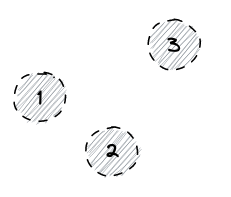
\includegraphics[width=0.5\textwidth]{d2n3_solvable.png}
    \label{fig:d2n3_solvable}
\end{figure}

\begin{figure}[h]
    \caption{Solvable example with $d=3$ and $N=4$}
    \centering
    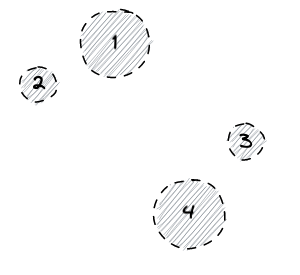
\includegraphics[width=0.5\textwidth]{d3n4_solvable.png}
    \label{fig:d3n4_solvable}
\end{figure}


It was not until a day of thinking and researching that I found these \href{https://people.csail.mit.edu/alinush/6.867-fall-2013/2013.10.22.w8.tu-lecture-13-generalization-part-2.pdf}{\underline{Slides}}\footnote{\url{https://people.csail.mit.edu/alinush/6.867-fall-2013/2013.10.22.w8.tu-lecture-13-generalization-part-2.pdf}} (Page 5) that confirmed my original answer.

\subsection{Using the bound from Exercise 3.d, determine the smallest upper-bound on the VC-dimension for decision stumps for dimensionalities $d ∈ \{1, 2, 3, 4, 5, 6, 7, 8, 1024, 2^{100}\}$}
\label{sec:2e}
I used the definition from the book \textit{Foundations of Machine Learning} \cite{foundations_of_machine_learning} for the upper-bound on the VC-Dimension

\textbf{Smallest upper-bound on VC-dimension}: To give an upper bound, we need to prove that no set $S$ of cardinality $N$ can be shattered

Since we know the maximum number of different labelings a data set of size $N$ in $d$ dimensions can get by means of decision stumps to be $2Nd$ (Section \ref{sec:2d}), and the total number of possible different labelings of a data set of size $N$ can get is $2^N$ (Section \ref{sec:2a}), we have to find the first case where $2Nd < 2^N$. In other words, find the first $N$ for which the classifier cannot create every possible labeling.

Since I could not find an analytical solution to this I decided to solve it programmatically. The results can be seen in Table \ref{tab:upper-bound-vc}. I've also added results for $d \in \{9, 10, 11, 12\}$ for Section \ref{sec:2e}.

\begin{table*}
    \begin{tabular}{|c|c|}
    \hline
    Dimensionality & Upper-bound on VC-Dimension \\ \hline
    1              & 2                            \\ \hline
    2              & 4                            \\ \hline
    3              & 4                            \\ \hline
    4              & 5                            \\ \hline
    5              & 5                            \\ \hline
    6              & 6                            \\ \hline
    7              & 6                           \\ \hline
    8              & 6                            \\ \hline

    9              & 6                            \\ \hline
    10              & 7                            \\ \hline
    11             & 7                            \\ \hline
    12              & 7                            \\ \hline

    
    1024           & 14                            \\ \hline
    $2^{100}$        & 107 \\
    \hline
    \end{tabular}
    \caption{Results for upper bounds on the VC Dimension}
    \label{tab:upper-bound-vc}
\end{table*}

To me one interesting thing about these results is that they did not seem to agree with some other results I had found online. \href{https://people.csail.mit.edu/alinush/6.867-fall-2013/2013.10.22.w8.tu-lecture-13-generalization-part-2.pdf}{\underline{These slides}}\footnote{\url{https://people.csail.mit.edu/alinush/6.867-fall-2013/2013.10.22.w8.tu-lecture-13-generalization-part-2.pdf}} mentions the growth should be proportional to $\log(d)$, which it is. But \href{http://courses.cms.caltech.edu/cs253/hw/hw2.pdf}{\underline{this homework assignment}}\footnote{\url{http://courses.cms.caltech.edu/cs253/hw/hw2.pdf}} gives an upper=bound on the VC dimension of $2(\log_2(d) + 1)$. I think they might have found an analytical solution to the upper-bound, but in doing so had to slightly increase it.

\subsection{Write a program that finds lower-bounds experimentally and that would even find the true VC-dimension given enough time (and a sufficient numerical precision). Provide a clear description for (possibly in terms of pseudo code) and reasoning behind the program. (Hint: given an arbitrary data set of of size N, you can of course always check if the class of decision stumps shatters it.)}
\label{sec:2f}

Once again the definition from the book \textit{Foundations of Machine Learning} \cite{foundations_of_machine_learning} for the lower-bound on the VC-Dimension is used

\textbf{Upper-bound on VC-dimension}: To give a lower bound, we need to show that a set $S$ of cardinality $N$ can be shattered

\begin{lstlisting}[language=Python, caption=Can Shatter Method, label={alg:shatter}]
def can_shatter(dataset):
    d = len(dataset[0])
    max_labelings = 2**len(dataset)
    # both are arrays of size 2
    min_values = np.min(dataset, axis=0)
    max_values = np.max(dataset, axis=0)

    found_labels = set()
    # iterate over dimension, lower_bound, upper_bound
    iterator = zip(range(d), min_values, max_values)
    for stump_dimension, start, end in iterator:
        for stump_boundary in range(start-1, end+1):
            # anything lower than the stump boundary gets True
            labeled = dataset[:, stump_dimension] <= stump_boundary
            found_labels.add(tuple(labeled))
            # inverse is always achievable
            found_labels.add(tuple(~labeled))
            # stop when we found the max number of possible labels:
            # dataset can be shattered
            if len(found_labels) == max_labelings:
                return True
    return False
\end{lstlisting}

The code for this can be seen in Algorithm \ref{alg:shatter}. I tried writing it out in pseudo code but this turned out to be almost the exact same as the Python code, so I think it's clearer add the original code with comments.

One thing that's good to explain is how I choose the locations of the decision boundaries. In my code the samples are always on integer coordinates (more on my sampling method later), so by iterating my decision boundary over all possible integers I am sure to get all possible labelings. It is of course not needed to go over every possible integer, so instead for each dimension I choose the decision boundary to be in:

\[ boundary \in \{lower\_bound - 1, lower\_bound, ..., upper\_bound\} \]

Here $lower\_bound$ and $upper\_bound$ are the lowest and highest value found for each dimension in the data set. 

I tried multiple methods of sampling the possible search space. A first question I had was how big should the space be. For example if there is only $3$ samples in $2$ dimensions it seems unneccesary to have these samples be in a space of size $1000x1000$. In some earlier experiments I noticed that for $d \leq 4$ I could find solutions for a space where each dimension has a max size of $d$. So this was often the starting size of my sample space, which I then increased if I thought it was needed.

For the sampling method itself I tried 2 methods, \textit{random} and \textit{enumeration}. A problem I ran into with both methods was the sheer size of the possible number of data sets. If we have $d=3$ and each dimension has a size of $3$ this gives $27$ possible points. Choosing 4 points from this (the upper-bound for $d=3$ found in Section \ref{sec:2e}) gives a total of 17550 possible data sets. This is still easy to enumerate, but the size grows rapidly. For $d=5$ and each dimension having a size of 5 there is $3125$ possible points. Choosing 5 from this gives $2.47e15$ possible data sets. Because the number of possible data sets grows so rapidly I decided to stick with random sampling.

\begin{lstlisting}[language=Python, caption=Dimensionality Check, label={alg:finder}]
def check_dimensionality(config):
    d, upper_bound, max_attempts = config
    # check from highest possible VD dimension first
    # this was if it is found we can immediately stop
    iterator = list(range(1, upper_bound+1))[::-1]
    for N in iterator:
        attempts = 0
        for data in generate_random_data(d, N):
            # just need to find a single dataset that can be shattered
            if can_shatter(data):
                print(f'Highest N for dimension {d} is: {N}')
                return
            attempts += 1
            if attempts >= max_attempts:
                break
    \end{lstlisting}

Finally Algorithm \ref{alg:shatter} was used in Algorithm \ref{alg:finder} to check multiple data set sizes to find the VC-dimension.

\subsection{Determine for every dimensionality $d ∈ \{1, 2, 3, . . . , 10, 11, 12\}$ the true VC-dimension and proof that, indeed, it is the actual VC-dimension for decision stump in spaces of that dimensionality. (Note: please be advised that you are not expected to completely crack this open(?) problem, but do have a go at it and see how far you can get in a reasonable amount of time. Hint: you probably can get some inspiration from the lower-bounds your program from 3.f finds.)}
\label{sec:2g}

\begin{table*}
    \begin{tabular}{|c|c|}
    \hline
    Dimensionality & Lower-bound on VC-Dimension \\ \hline
    1              & \textbf{2}                            \\ \hline
    2              & 3                            \\ \hline
    3              & \textbf{4}                            \\ \hline
    4              & 4                            \\ \hline
    5              & \textbf{5}                            \\ \hline
    6              &    5                         \\ \hline
    7              & 5                           \\ \hline
    8              & 5                            \\ \hline
    9              & 5                            \\ \hline
    10              & 5                            \\ \hline
    11             &  6                          \\ \hline
    12              &  6                           \\ \hline
    \end{tabular}
    \caption{Results for experimentally found lower bounds on the VC Dimension}
    \label{tab:experiment-lower-bound-vc}
\end{table*}

I used the method described in Section \ref{sec:2f} to experimentally find lower-bounds on the VC dimension. Results for this can be seen in Table \ref{tab:experiment-lower-bound-vc}. The boldfaced values are where the lower and upper bound match. To find these values I ran tests with the algorithm shown in Algorithm \ref{alg:finder} using 1000000 attempts each time. I varied the size per dimension from $N$ to $16N$.

% In my experiments I found the VC-dimension for $d=2$ to be most likely 3. I then found \href{http://www.cs.cmu.edu/~aarti/Class/10701_Spring14/slides/LearningTheoryII.pdf}{\underline{this presentation}}\footnote{\url{http://www.cs.cmu.edu/~aarti/Class/10701_Spring14/slides/LearningTheoryII.pdf}} that shows a proof that I will try to explain in my own words:

\bibliographystyle{plain}
\bibliography{refs}

\end{document}